\begin{center}
    \textbf{\textbf{Cardinalidad de la consulta}}
\end{center}

Considera las siguientes relaciones:
\begin{table}[H]
    \centering
    \setlength{\tabcolsep}{10pt} % Ajusta el espacio entre tablas
    \begin{minipage}{0.4\textwidth}
        \centering
        \rowcolors{2}{blue!25}{white}
        \begin{tabular}{|c|c|}
        \hline
        \rowcolor{blue!50}
        \textcolor{white}{\textbf{A}} & \textcolor{white}{\textbf{B}} \\ \hline
        \textbf{1} & x \\ \hline
        \textbf{2} & y \\ \hline
        \textbf{2} & z \\ \hline
        \textbf{3} & x \\ \hline
        \textbf{9} & a \\ \hline
        \end{tabular}
        \caption{R}
    \end{minipage}
    \hspace{2cm} % Espacio entre las dos tablas
    \begin{minipage}{0.4\textwidth}
        \centering
        \rowcolors{2}{blue!25}{white}
        \begin{tabular}{|c|c|c|}
        \hline
        \rowcolor{blue!50}
        \textcolor{white}{\textbf{B}} & \textcolor{white}{\textbf{C}} & \textcolor{white}{\textbf{D}} \\ \hline
        x & 0 & 3 \\ \hline
        y & 2 & 1 \\ \hline
        y & 3 & 3 \\ \hline
        w & 3 & 0 \\ \hline
        y & 4 & 2 \\ \hline
        \end{tabular}
        \caption{S}
    \end{minipage}
\end{table}

Para las siguientes expresiones de álgebra relacional, completa la tabla con el número de tuplas que cada una de ellas
produce utilizando las relaciones R y S. Deberás indicar las tablas resultantes en cada caso.

% group: Group1 

% R = {
% A:number, B:string
% 1,  x
% 2,  y
% 2,  z
% 3,  x
% 9,  a
% }

% S = {
% B:string, C:number, D:number
% x, 0, 3
% y, 2, 1
% y, 3, 3
% w, 3, 0
% y, 4, 2
% }


\begin{longtable}{|p{4.3cm}|p{12cm}|}
    \hline
    \rowcolor{blue!50}
    \textcolor{white}{\textbf{Expresión}} & \textcolor{white}{\textbf{Cardinalidad del resultado}} \\ \hline
    \textbf{$R \times S$} & 
    Al ser un producto cartesiano se tienen 5 x 5 = 25 tuplas. 

    \begin{center}
        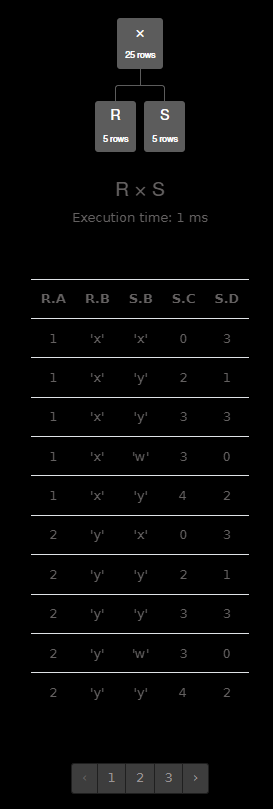
\includegraphics[height=12cm]{../resources/pregunta1/1.1.png}
    \end{center}
    \\ \hline
    
    \textbf{$R \bowtie D > A \ S$} & 
    Esta hace un join natural donde D es mayor que A, resulta en 7 tuplas : 

    \begin{center}
        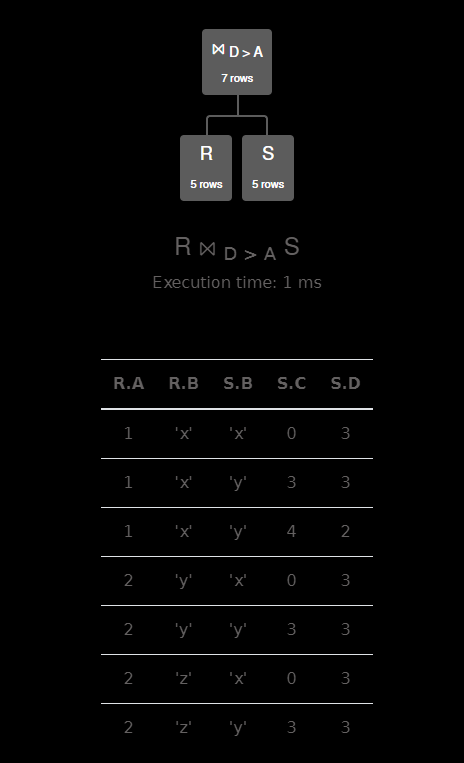
\includegraphics[height=8cm]{../resources/pregunta1/1.2.png}
    \end{center}
    \\ \hline
    
    \textbf{$R \leftouterjoin S$} & 
    Se selecciona la relación R y se junta con S usando su columna en comun, si no hay coincidencia en S se añade un null, resultando en 7 tuplas:
    
    \begin{center}
        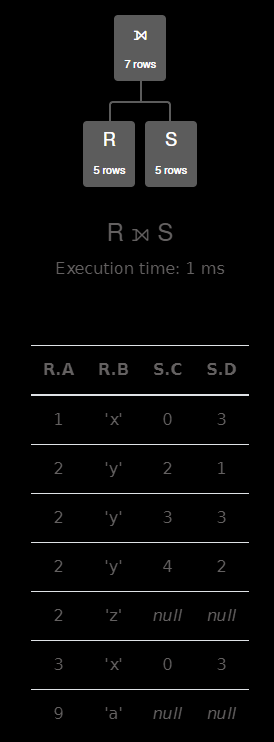
\includegraphics[height=8cm]{../resources/pregunta1/1.3.png}
    \end{center}
    \\ \hline
    
    \textbf{$R \rightouterjoin S$} & 
    Se selecciona la relación S y se junta con R usando su columna en comun, si no hay coincidencia en R se añade un null, resultando en 6 tuplas:

    \begin{center}
        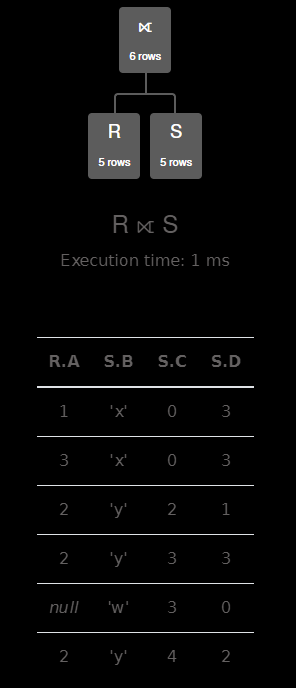
\includegraphics[height=8cm]{../resources/pregunta1/1.4.png}
    \end{center}
    \\ \hline
    
    \textbf{$R \bowtie A = D \ S$} & 
    Al ser un thetha join, se seleccionan las tuplas que cumplan con la condición, en este caso que A sea igual a D (por cada de A buscas cuantos D son iguales), se obtienen 5 tuplas:

    \begin{center}
        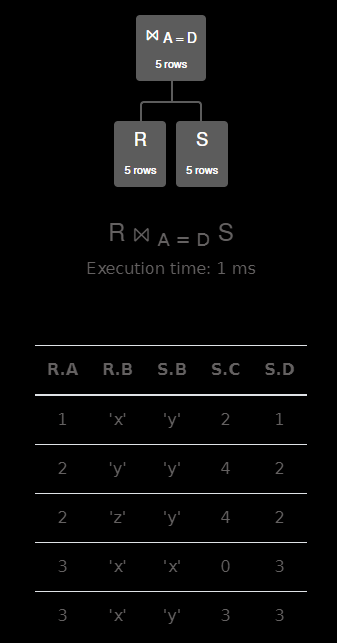
\includegraphics[height=8cm]{../resources/pregunta1/1.5.png}
    \end{center}
    \\ \hline
    
    \textbf{$\rho \ C \leftarrow A \ R \bowtie S$} & 
    Se renombra la columna A de R a C y se hace un join natural con S, se regresa donde C sea igual a A y como comparten B tambien debe ser igual, resultando en 1 tupla:

    \begin{center}
        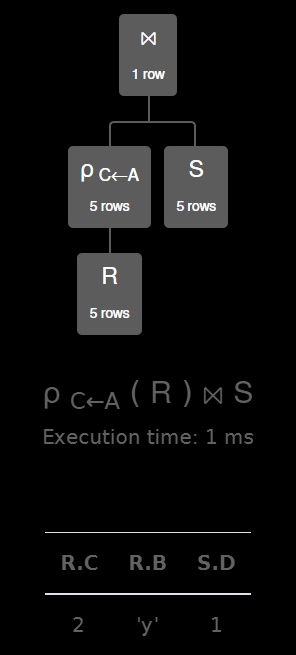
\includegraphics[height=8cm]{../resources/pregunta1/1.6.png}
    \end{center}
    \\ \hline
    
    \textbf{$\pi B (R) - \pi B (\sigma C \geq 2 (S))$} & 
    Se selecciona de S las tuplas donde C es mayor o igual a 2, se seleccionan las diferentes B de la consulta anterior; se toman las diferentes B de R y se restan la primera consulta, resultando en 3 tuplas:

    \begin{center}
        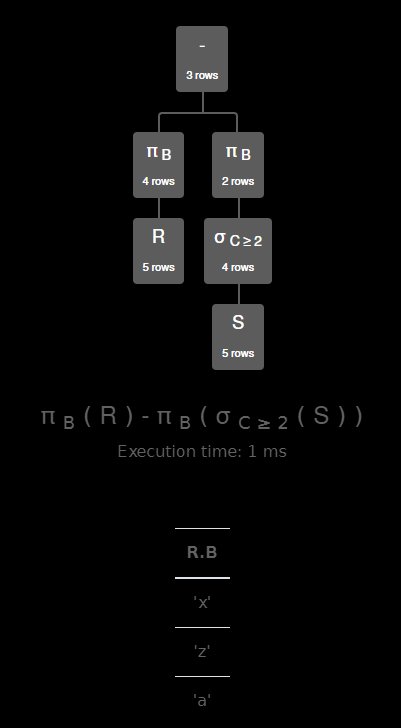
\includegraphics[height=8cm]{../resources/pregunta1/1.7.png}
    \end{center}
    \\ \hline
    
    \textbf{$\pi A (R) \cap \rho A \leftarrow D \ (\pi D (S))$} & 
    Selecciona las diferentes A de R y se intersectan con las diferentes D de S ahora renombradas a A, resultando en 3 tuplas:

    \begin{center}
        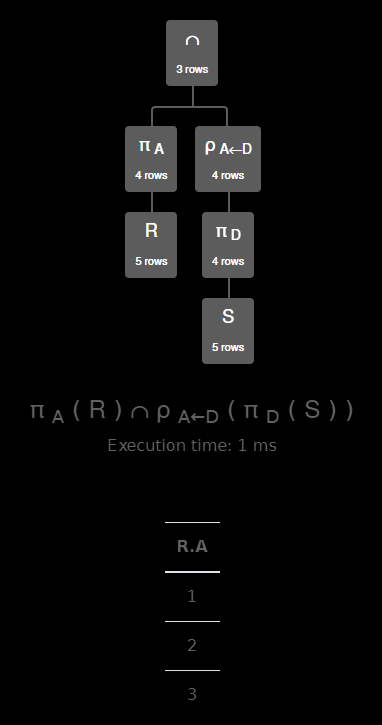
\includegraphics[height=8cm]{../resources/pregunta1/1.8.png}
    \end{center}
    \\ \hline
    
    \textbf{$\pi D (S) \bowtie S.D > R.A \ R$} & 
    Selecciona las diferentes D de S y se hace un join natural con S, se seleccionan las tuplas donde D es mayor que A de R, resultando en 4 tuplas:

    \begin{center}
        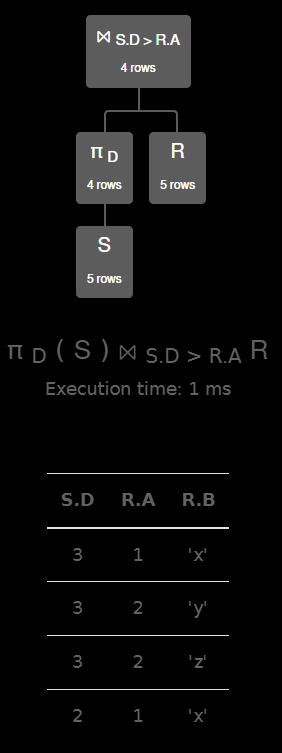
\includegraphics[height=8cm]{../resources/pregunta1/1.9.png}
    \end{center}
    \\ \hline
    
    \textbf{$\gamma A; \text{count}(B) \to t (R \bowtie S)$} & 
    Empezamos haciendo el natural join de R y S donde B es igual, si falta alguno ponemos null, agrupamos las filas resultantes por el atributo A de R usando la funcion de agregacion que cuenta el numero de ocurrencias de cada valor B en la relacion R (B era ambibguo pues ambos tienen B) por cada grupo de A, el resultado se guarda en una columna llamada t, al final salen 5 tuplas: (una por cada tipo de A)

    \begin{center}
        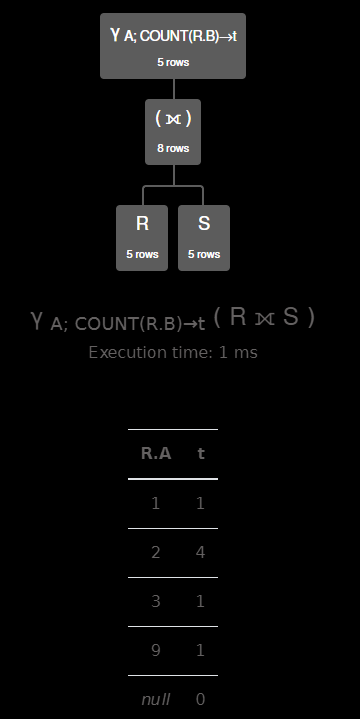
\includegraphics[height=8cm]{../resources/pregunta1/1.10.png}
    \end{center}
    \\ \hline
\end{longtable}
 
\vspace{1cm}
